%%%%%%%%%%%%%%%%%%%%%%%%%%%%%%%%%%%%%%%%%
%% Data section
\section{Data and Genetic Context}
\label{sec:data}
This paper draws on data from the UK Biobank, a large-scale cohort study of the British population with both rich socioeconomic measures and detailed genetic data.
I construct the Education PolyGenic Index (Ed PGI) summarising each participant's genetic predisposition toward educational attainment, and impute parental PGI values using genetic data from siblings.
Together, these data enable a within-family research design that separates the role of inherited genetic factors from the shared family environment in shaping socioeconomic outcomes.

\subsection{UK Biobank (UKB)}
\label{sec:data-UKB}
The UK Biobank (UKB) is a large-scale prospective cohort study comprising approximately half a million members of the British public, recruited between 2006 and 2010.
Letters were sent to a random sample of addresses in the National Health Service registry, and the final UKB data represent voluntary respondents.
%\footnote{
%    The UKB may not be representative of the entire UK population, as it only represents willing respondents.
%    As such, the findings of this paper should only be taken as internally valid among the UKB respondents, and the sibling analysis sample described.
%}
Participants, aged 40-69 years at recruitment, underwent comprehensive baseline assessments, were asked many questions for socioeconomic information either by interview, automated survey answers, or follow-up sessions.
Key socioeconomic variables include educational attainment (measured in education qualifications), household income brackets, employment status, and industry of employment.
See \cite{sudlow2015uk} for a full description of the UKB organisation and data.

\begin{table}[!htp]
    \vskip-0.75cm
    \singlespacing
    \centering
    \small
    \caption{Descriptive Statistics, UKB.}
    \vskip-0.25cm
    \begin{tabular}{l c c c c}
        \\[-1.8ex]\hline \hline \\[-1.8ex] 
            & \multicolumn{2}{c}{Analysis sample}
            & \multicolumn{2}{c}{Entire sample} \\
        \cmidrule(lr){2-3} \cmidrule(lr){4-5}
        & Mean & SD & Mean & SD \\
        \\[-1.8ex]\hline \\[-1.8ex]
        % latex table generated in R 4.5.1 by xtable 1.8-4 package
% Tue Jul  1 13:00:33 2025
 \\[-1.8ex] \textit{Demographics:} &   &   &   &   \\ 
  Male & 0.45 & 0.50 & 0.46 & 0.50 \\ 
  Age & 53.57 & 6.48 & 56.55 & 8.09 \\ 
  Ethnicity $=$ European & 1.00 & 0.00 & 0.82 & 0.38 \\ 
  Any siblings also in UKB? & 1.00 & 0.00 & 0.08 & 0.28 \\ 
  Count of siblings in UKB & 1.09 & 0.33 & 0.09 & 0.32 \\ 
  \\[-1.8ex]\hline \\[-1.8ex] \textit{Education:} &   &   &   &   \\ 
  Ed PGI & 0.02 & 1.00 & -0.00 & 1.00 \\ 
  Ed PGI, parental mean & -0.04 & 0.75 &   &   \\ 
  Education years & 13.86 & 3.33 & 13.71 & 3.49 \\ 
  Qualification, University degree & 0.33 & 0.47 & 0.33 & 0.47 \\ 
  Qualification, A-Levels & 0.46 & 0.50 & 0.45 & 0.50 \\ 
  Qualification, GCSEs & 0.77 & 0.42 & 0.71 & 0.45 \\ 
  Qualification, Professional degree & 0.31 & 0.46 & 0.29 & 0.45 \\ 
  Qualification, Vocational degree & 0.25 & 0.43 & 0.19 & 0.39 \\ 
  Qualification, No official qualifications & 0.12 & 0.33 & 0.17 & 0.38 \\ 
  \\[-1.8ex]\hline \\[-1.8ex] \textit{Labour Market Outcomes:} &   &   &   &   \\ 
  Occupation hourly wage, \pounds & 20.01 & 9.03 & 20.91 & 9.51 \\ 
  Occupation annual income, thousands \pounds & 28.67 & 18.85 & 30.40 & 19.94 \\ 
  Average hours worked, per week & 34.73 & 12.58 & 35.31 & 12.70 \\ 
  Household income, $< \pounds 18k$ & 0.10 & 0.29 & 0.20 & 0.40 \\ 
  Household income, $\pounds 18-31k$ & 0.22 & 0.41 & 0.22 & 0.41 \\ 
  Household income, $\pounds 31-52k$ & 0.30 & 0.46 & 0.22 & 0.42 \\ 
  Household income, $\pounds 52-100k$ & 0.24 & 0.43 & 0.17 & 0.38 \\ 
  Household income, $\pounds 100k <$ & 0.06 & 0.23 & 0.05 & 0.21 \\ 
  
        \\[-1.8ex]\hline \\[-1.8ex]
        Observations
            & \input{sections/tables/ukb-analysis-count.tex} &
            & \input{sections/tables/ukb-total-count.tex} & \\
        \\[-1.8ex]\hline \\[-1.8ex]
    \end{tabular}
    \vspace{-0.25cm}
    \label{tab:ukb-summary}
    \justify
    \footnotesize
    \textbf{Note:}
    This table shows the Mean and Standard Deviation (SD) of UKB variables, comparing the analysis subsample and the entire UKB sample.
    The analysis sample refers to individuals with at least one family member also included in the UKB (sibling or parent), have non-missing education and labour market occupation codes, and are of European ancestry.
    All genetic variables are coded as missing among those who report ancestry that is not European.
\end{table}

The UKB collected detailed information on educational qualifications, including completion of primary school, GCSEs (typically completed at age 16), A-Levels (completed at age 18), and completion of an higher education degree.
I convert these qualifications into education years based on each participant's highest reported qualification, following the International Standard Classification of Education.\footnote{
    British vocational degrees are inconsistently coded by the International Standard Classification of Education.
    I follow \cite{okbay2022polygenic}, and assign education years as the age they reported leaving full-time education minus five, among those with a vocational degree as their highest qualification.
}
While the UKB collected household income data, this information was recorded only in categorical bins; I assign midpoint imputed values and update to 2024 GBP for a coarse measure of household income.
To accompany these measures with a finer measure of income, I also calculate occupation income.
I construct an individual-level income measure using participants' 4-digit Standard Occupational Classification (SOC) codes.
Specifically, I impute occupation-based wages by estimating hourly earnings for each SOC category using data from the British Annual Survey of Hours and Earnings, conditional on age, gender, and year.\footnote{
    This approach uses replication data files provided by \cite{kweon2025associations}, also used by \cite{carvalho2024genetics}; see \appendixref{appendix:pgi-impute}.
}
This approach provides a more granular and continuous measure of economic status than the categorical household income variable.
I create the annual occupation income by multiplying this by the number of hours they reported working, times 52 weeks in the year.
This gives \input{sections/tables/ukb-total-count.tex}individuals in the UKB, with non-missing data in relevant variables. 


\begin{figure}[!h]
    \centering
    \singlespacing
    \caption{Distribution of UKB Education Measures.}
    \begin{subfigure}[b]{0.495\textwidth}
        \centering
        \caption{Education Years.}
        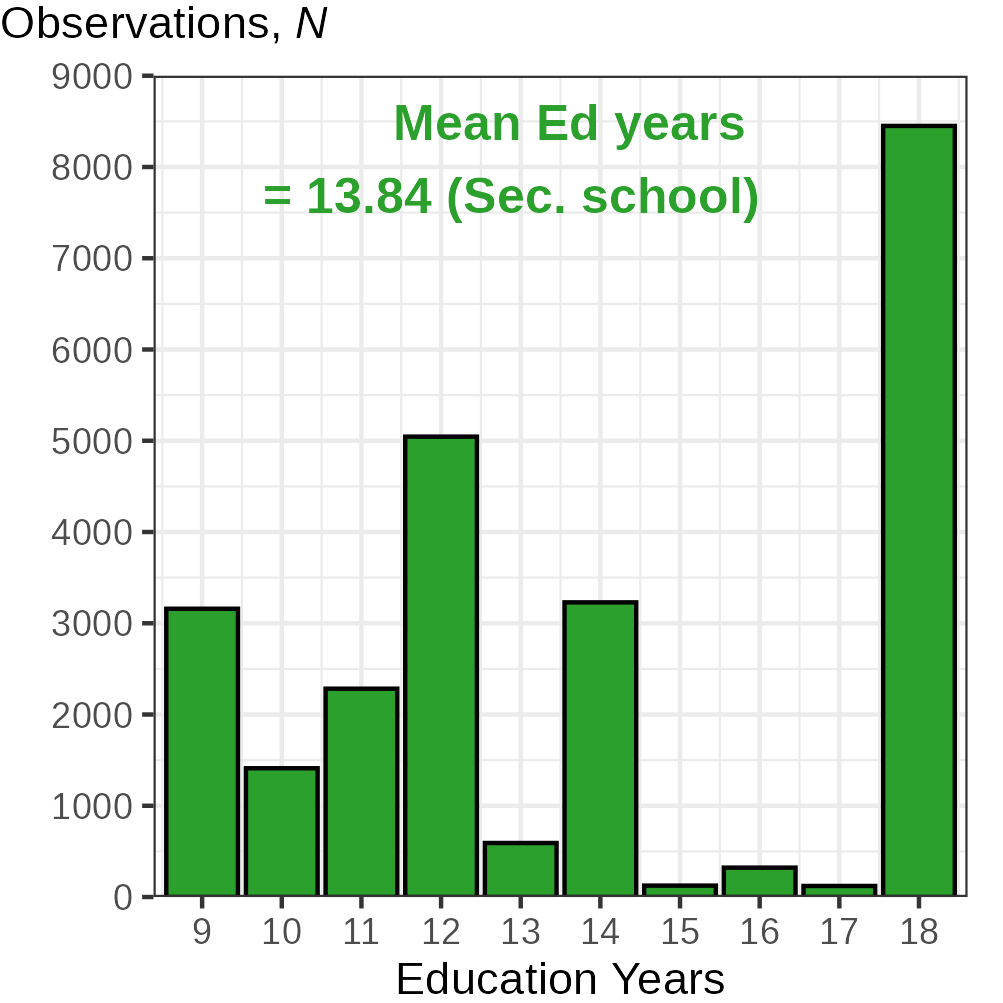
\includegraphics[width=\textwidth]{sections/figures/edyears-hist.png}
        \label{fig:edyears-hist}
    \end{subfigure}
    \begin{subfigure}[b]{0.495\textwidth}
        \centering
        \caption{Education Years $+$ Income.}
        
\includegraphics[width=\textwidth]{sections/figures/edyears-earnings.png}
        \label{fig:edyears-earnings}
    \end{subfigure}
    \label{fig:ukb-edyears-hist}
    \vspace{-1cm}
    \justify
    \footnotesize
    \textbf{Note}:
    The left plot shows the observation count in the UKB analysis sample with each number of reported education years, coded from education qualifications.
    The right plot shows the mean occupation imputed annual income for each level of education years, with a line of best fit calculated from a linear regression (with annual income measured in a log specification); the slope refers to the estimated coefficient from this linear regression.
\end{figure}

For the purposes of this study, the primary analysis sample is restricted to those with at least one family member, sibling or parent,\footnote{
    The UKB does not personally identify participants, nor their family members, so I follow the genetic literature by identifying family clusters by measures of genetic similarity.
    \appendixref{appendix:identifying-families} further describes the family definitions in the UKB. 
}
also enrolled in the UKB, and non-missing data in occupation code plus education qualifications.
This gives \input{sections/tables/ukb-analysis-count.tex}individuals in the UKB. 
The presence of multiple family members within the dataset provides a unique opportunity to control for shared genetic factors that might otherwise bias estimates in standard cross-sectional analyses.

The analysis sample is also restricted to individuals who report to have primarily European ancestry.
The genetic measures used in this paper have generally been constructed from primarily white, European descended populations, and have little predictive power out of sample, so are only relevant in this subsample.
It is an unfortunate fact that systematic genetic measures, such as those considered in this paper, have only been constructed from Biobank samples where the vast majority are white and/or European descended; see \cite{martin2017human} for a further discussion.
A limitation of this study is that its results only apply to this subset of the UKB population.

The only notable differences between the analysis subsample and the entire UKB participant sample are that the analysis sample has more siblings, and is entirely European descended; no other variables are significantly different for the analysis subsample.
\autoref{tab:ukb-summary} summarises the UKB data, for the analysis sample and among the entire UKB sample.
\autoref{fig:ukb-edyears-hist} summarises the correlation between education years and occupation coded income.

\subsection{Education PolyGenic Index (Ed PGI)}
\label{sec:ed-pgi}
UKB participants also provided saliva samples that were subsequently genotyped, producing standardised genetic data files for statistical analysis of the relationship between genetics and outcomes.

While genetic data provide rich information about individual variation, the relationship between specific genes and social outcomes like education is extraordinarily complex.
The biological pathways from DNA to observable traits remain largely opaque --- the exact relationship between a single gene, its resulting protein (or its moderating role), and the resulting outcomes are only known for a small number of genes in the human genome.
For example, a single gene (and its recessive variant) is known to lead to a protein which does not break down the by-products of alcohol digestion; individuals with this genetic variant generally do not drink alcohol at all because of the biological limit on digestion \citep{millwood2023alcohol}.
Complex social behaviours, on the other hand, have no single gene with a known biological pathway, so cannot be summarised with one single gene, nor single biological pathway.
Instead, complex social behaviours are a result on thousands of genes, and their interactions with the environment --- they are polygenic.

Rather than attempting to trace all of these intricate biological mechanisms, researchers have developed PolyGenic Indices (PGIs) as dimensional reduction tools that summarise the statistical relationship between thousands of genetic variants and outcomes of interest.
This statistical aggregation is particularly valuable because individual genetic variants typically have tiny associations with social outcomes like educational attainment --- often explaining less than 0.01\% of the variation.
However, by combining information across thousands of genetic variants, each contributing a small predictive association, PGIs can capture meaningful predictive power of genes for some social outcomes.
These indices are fundamentally correlational measures: they capture statistical associations between genetic variants and outcomes observed in large samples, not well understood biological pathways.

The Education PGI (Ed PGI) is the PolyGenic Index built to predict years of completed education, calculated from weights derived from a Genome-Wide Association Study (GWAS), which analysed the correlation between genetic variants and education years.
In a GWAS, researchers test the correlation between each Single Nucleotide Polymorphism (SNP) --- a one-letter change in the DNA sequence at a specific location --- and the outcome of interest \citep{uffelmann2021genome}.
I use the weights calculated in the GWAS conducted by \cite{okbay2022polygenic}, which used a sample of over 3 million individuals of European ancestry, primarily from 23\&Me data.

The Ed PGI is defined as the weighted sum of whether individual $i$ has the relevant SNP at each DNA location $j$,
\[ Z_i = \sum_{j = 1}^{J} w_j x_{i,j} \]
where $w_j$ are the Ed PGI weights (provided in the supplementary data to \citealt{okbay2022polygenic}), and $x_{i,j}$ is an allele count --- whether individual $i$ has the relevant SNP at DNA location $j$.\footnote{
    Every person has two copies of each chromosome, so that $x_{i,j}$ takes values 0, 1, 2 corresponding to how many copies of the SNP individual $i$ has inherited.
    The genetics literature has generally accepted that complex social behaviours are explained by additive effects (see \citealt{hill2008data}), and \cite{okbay2022polygenic} found little evidence for dominance in the Ed PGI SNPs, so that the Ed PGI makes sense as a weighted sum.
}
The \cite{okbay2022polygenic} GWAS found that around 4,000 individual SNPs were significant in predicting education years, after passing a battery of biostatistical tests and finding no evidence for significant interactions.
The resulting Ed PGI is standardised to have mean zero and standard deviation one within the entire sample, making it interpretable as the number of standard deviations from the population mean.
The Ed PGI captures approximately 12--15\% of the variation in educational attainment, making it one of the most predictive PGIs for any complex behavioural trait to date.

\begin{figure}[!h]
    \centering
    \singlespacing
    \caption{Distribution of Education PolyGenic Index (Ed PGI).}
    \begin{subfigure}[b]{0.495\textwidth}
        \centering
        \caption{Ed PGI.}
        
\includegraphics[width=\textwidth]{sections/figures/edpgi-hist.png}
        \label{fig:edpgi-hist}
    \end{subfigure}
    \begin{subfigure}[b]{0.495\textwidth}
        \centering
        \caption{Ed PGI $+$ Education Years, Bin Scatter.}
        
\includegraphics[width=\textwidth]{sections/figures/edpgi-edyears.png}
        \label{fig:edpgi-edyears}
    \end{subfigure}
    \label{fig:ukb-hist}
    \vspace{-1cm}
    \justify
    \footnotesize
    \textbf{Note}:
    The left plot shows a kernel density estimate for the distribution of the Ed PGI among the UKB analysis sample.
    Ed PGI is normalised to have mean 0 and standard deviation 1 among the entire UKB sample; it is roughly normally distributed regardless of this normalisation.
    The right plot shows a bin scatter, visualising a (semi-parametric) correlation between the Ed PGI and education years.
    The slope refers to the estimated coefficient from a linear regression between the Ed PGI and education years.
\end{figure}

If education had no relationship with SNP variants, then we would expect the correlation between the Ed PGI and education years to be indistinguishable from zero; it is, however, highly correlated with education years in the UKB analysis sample.
A one standard deviation increase in the Ed PGI is associated with 0.93 extra education years (standard error 0.02), with an $R^2$ value of 0.10 for the raw regression of education years on Ed PGI.
It is roughly normally distributed, with standard deviation normalised to 1.
This distribution is not surprising, as the Ed PGI is the weighted sum of a few thousand binary variables, so we should expect convergence towards a normal distribution among the population.
The main takeaway is that the correlation between a summary measure of genetic values is strong, and has meaningful predictive power for education years.

The Ed PGI is not the only PGI that can be constructed.
Following the same methodology, I construct additional PGIs for seven health-related traits that may confound the relationship between genetics and socioeconomic outcomes: asthma, bipolar disorder, Body Mass Index (BMI), height, schizophrenia, and type 2 diabetes.
Each PGI is calculated using the same approach as the Ed PGI --- taking weights from a published GWAS, conducted on independent populations, and computing weighted sums of the relevant genetic variants in the UKB data.
These other PGIs serve as control variables in my analysis for two reasons.
First, genetic variants often exhibit pleiotropy, meaning a single variant can influence multiple traits simultaneously.
For instance, genetic variants associated with education might also affect other factors (e.g., mental health conditions), which could independently influence labour market outcomes.
Second, systematic differences in gene frequencies across ancestry groups can create spurious correlations between any PGI and outcomes if health conditions vary across these groups for unrelated reasons.

\subsection{Imputing Parental PGIs from Siblings}
\label{sec:pgi-impute}
It would be ideal if the UKB contained genetic information for the parents of every UKB participant.
While there are 6,239 participants with a parent also included in the UKB, there are only 72 with both parents.
To overcome this missing data problem, I also use siblings' genetic data to impute the mean parental PGIs from the sample of \input{sections/tables/ukb-analysis-count.tex} participants with at least one family member (parent or sibling) also in the UKB --- the analysis sample described above.
The majority of this analysis sample have genetic data on one sibling member, so I refer to this as sibling imputation.

\begin{figure}[!h]
    \centering
    \singlespacing
    \caption{Imputing One SNP for Parents from Sibling Data.}
    \label{fig:pgi-imputing}
    % ---- IBD0 ----
% Code for the TikZ picture showing how the Young et al (2022) imputation procedure works.
\begin{subfigure}[b]{0.25\textwidth}
    \centering
    \begin{tikzpicture}
        % Draw parental nodes
        \node[state,dashed,gray] (mother) at (-1, 3) {?};
        \node[state,dashed,gray] (father) at (1, 3)  {?};
        \node [above=0.25cm of mother] {\textcolor{orange}{Mother}};
        \node [above=0.25cm of father] {\textcolor{blue}{Father}};
        % Draw individual, and their sibling, nodes.
        \node[state] (individual) [below=1cm of mother] {1};
        \node[state] (sibling)    [below=1cm of father] {1};
        \node [below=0.25cm of individual] {\textcolor{ForestGreen}{Child}};
        \node [below=0.25cm of sibling]    {\textcolor{purple}{Sibling}};
        % Draw the family connections
        \coordinate (betweenparents) at ($(mother)!0.5!(father)$);
        \coordinate (aboveindividual) at ($(mother)!0.5!(individual)$);
        \coordinate (abovesibling) at ($(father)!0.5!(sibling)$);
        \coordinate (aboveboth) at ($(aboveindividual)!0.5!(abovesibling)$);
        \path[-,dashed,gray] (mother) edge (father);
        \path[-,dashed,gray] (betweenparents) edge (aboveboth);
        \path[-] (aboveindividual) edge (abovesibling);
        \path[-] (aboveindividual) edge (individual);
        \path[-] (abovesibling) edge (sibling);
        % Bridge to the others
        \node[scale=2] [right=1cm of abovesibling]{$\Rightarrow$};
        \node [left=3.5cm of abovesibling]{IB0:};
    \end{tikzpicture}
\end{subfigure}
\hskip3cm
\begin{subfigure}[b]{0.25\textwidth}
    \centering
    \begin{tikzpicture}
        % Draw parental nodes
        \node[state] (mother) at (-1, 3) {1};
        \node[state] (father) at (1, 3)  {1};
        \node [above=0.25cm of mother] {\textcolor{orange}{Mother}};
        \node [above=0.25cm of father] {\textcolor{blue}{Father}};
        \node [color=white,below=0.25cm of individual] {Child};
        \node [color=white,below=0.25cm of sibling]    {Sibling};
        % Draw individual, and their sibling, nodes.
        \node[color=white,state] (individual) [below=1cm of mother] {1};
        \node[color=white,state] (sibling)    [below=1cm of father] {0};
        % Draw the family connections
        \coordinate (betweenparents) at ($(mother)!0.5!(father)$);
        \coordinate (aboveindividual) at ($(mother)!0.5!(individual)$);
        \coordinate (abovesibling) at ($(father)!0.5!(sibling)$);
        \coordinate (aboveboth) at ($(aboveindividual)!0.5!(abovesibling)$);
        \path[-,dashed,gray] (mother) edge (father);
        \path[-,dashed,gray] (betweenparents) edge (aboveboth);
        %\path[-] (aboveindividual) edge (abovesibling);
        %\path[-] (aboveindividual) edge (individual);
        %\path[-] (abovesibling) edge (sibling);
        \node [below=0.5cm of aboveboth] {Mean parent SNP $= 1$};
    \end{tikzpicture}
\end{subfigure}

% ---- IBD1 ----
% Code for the TikZ picture showing how the Young et al (2022) imputation procedure works.
\begin{subfigure}[b]{0.25\textwidth}
    \centering
    \begin{tikzpicture}
        % Draw parental nodes
        \node[state,dashed,gray] (mother) at (-1, 3) {?};
        \node[state,dashed,gray] (father) at (1, 3)  {?};
        \node [above=0.25cm of mother] {\textcolor{orange}{Mother}};
        \node [above=0.25cm of father] {\textcolor{blue}{Father}};
        % Draw individual, and their sibling, nodes.
        \node[state] (individual) [below=1cm of mother] {2};
        \node[state] (sibling)    [below=1cm of father] {1};
        \node [below=0.25cm of individual] {\textcolor{ForestGreen}{Child}};
        \node [below=0.25cm of sibling]    {\textcolor{purple}{Sibling}};
        % Draw the family connections
        \coordinate (betweenparents) at ($(mother)!0.5!(father)$);
        \coordinate (aboveindividual) at ($(mother)!0.5!(individual)$);
        \coordinate (abovesibling) at ($(father)!0.5!(sibling)$);
        \coordinate (aboveboth) at ($(aboveindividual)!0.5!(abovesibling)$);
        \path[-,dashed,gray] (mother) edge (father);
        \path[-,dashed,gray] (betweenparents) edge (aboveboth);
        \path[-] (aboveindividual) edge (abovesibling);
        \path[-] (aboveindividual) edge (individual);
        \path[-] (abovesibling) edge (sibling);
        % Bridge to the others
        \node[scale=2] [right=1cm of abovesibling]{$\Rightarrow$};
        \node [left=3.5cm of abovesibling]{IB1:};
    \end{tikzpicture}
\end{subfigure}
\hskip3cm
\begin{subfigure}[b]{0.25\textwidth}
    \centering
    \begin{tikzpicture}
        % Draw parental nodes
        \node[state] (mother) at (-1, 3) {1};
        \node[state,dashed,gray] (father) at (1, 3)  {?};
        \node [above=0.25cm of mother] {\textcolor{orange}{Mother}};
        \node [above=0.25cm of father] {\textcolor{blue}{Father}};
        \node [color=white,below=0.25cm of individual] {Child};
        \node [color=white,below=0.25cm of sibling]    {Sibling};
        % Draw individual, and their sibling, nodes.
        \node[color=white,state] (individual) [below=1cm of mother] {2};
        \node[color=white,state] (sibling)    [below=1cm of father] {1};
        % Draw the family connections
        \coordinate (betweenparents) at ($(mother)!0.5!(father)$);
        \coordinate (aboveindividual) at ($(mother)!0.5!(individual)$);
        \coordinate (abovesibling) at ($(father)!0.5!(sibling)$);
        \coordinate (aboveboth) at ($(aboveindividual)!0.5!(abovesibling)$);
        \path[-,dashed,gray] (mother) edge (father);
        \path[-,dashed,gray] (betweenparents) edge (aboveboth);
        %\path[-] (aboveindividual) edge (abovesibling);
        %\path[-] (aboveindividual) edge (individual);
        %\path[-] (abovesibling) edge (sibling);
        \node [right=0.4cm of father] {or};
        \node [below=0.5cm of aboveboth] {Mean = $\frac{1 + f}{2}$};
    \end{tikzpicture}
\end{subfigure}
\begin{subfigure}[b]{0.2\textwidth}
    \centering
    \begin{tikzpicture}
        % Draw parental nodes
        \node[state] (mother) at (-1, 3) {2};
        \node[state,dashed,gray] (father) at (1, 3)  {?};
        \node [above=0.25cm of mother] {\textcolor{orange}{Mother}};
        \node [above=0.25cm of father] {\textcolor{blue}{Father}};
        \node [color=white,below=0.25cm of individual] {Child};
        \node [color=white,below=0.25cm of sibling]    {Sibling};
        % Draw individual, and their sibling, nodes.
        \node[color=white,state] (individual) [below=1cm of mother] {1};
        \node[color=white,state] (sibling)    [below=1cm of father] {0};
        % Draw the family connections
        \coordinate (betweenparents) at ($(mother)!0.5!(father)$);
        \coordinate (aboveindividual) at ($(mother)!0.5!(individual)$);
        \coordinate (abovesibling) at ($(father)!0.5!(sibling)$);
        \coordinate (aboveboth) at ($(aboveindividual)!0.5!(abovesibling)$);
        \path[-,dashed,gray] (mother) edge (father);
        \path[-,dashed,gray] (betweenparents) edge (aboveboth);
        %\path[-] (aboveindividual) edge (abovesibling);
        %\path[-] (aboveindividual) edge (individual);
        %\path[-] (abovesibling) edge (sibling);
        \node [below=0.5cm of aboveboth] {Mean = $\frac{2 + f}{2}$};
    \end{tikzpicture}
\end{subfigure}

% ---- IBD0 ----
% Code for the TikZ picture showing how the Young et al (2022) imputation procedure works.
\begin{subfigure}[b]{0.25\textwidth}
    \centering
    \begin{tikzpicture}
        % Draw parental nodes
        \node[state,dashed,gray] (mother) at (-1, 3) {?};
        \node[state,dashed,gray] (father) at (1, 3)  {?};
        \node [above=0.25cm of mother] {\textcolor{orange}{Mother}};
        \node [above=0.25cm of father] {\textcolor{blue}{Father}};
        % Draw individual, and their sibling, nodes.
        \node[state] (individual) [below=1cm of mother] {1};
        \node[state] (sibling)    [below=1cm of father] {1};
        \node [below=0.25cm of individual] {\textcolor{ForestGreen}{Child}};
        \node [below=0.25cm of sibling]    {\textcolor{purple}{Sibling}};
        % Draw the family connections
        \coordinate (betweenparents) at ($(mother)!0.5!(father)$);
        \coordinate (aboveindividual) at ($(mother)!0.5!(individual)$);
        \coordinate (abovesibling) at ($(father)!0.5!(sibling)$);
        \coordinate (aboveboth) at ($(aboveindividual)!0.5!(abovesibling)$);
        \path[-,dashed,gray] (mother) edge (father);
        \path[-,dashed,gray] (betweenparents) edge (aboveboth);
        \path[-] (aboveindividual) edge (abovesibling);
        \path[-] (aboveindividual) edge (individual);
        \path[-] (abovesibling) edge (sibling);
        % Bridge to the others
        \node[scale=2] [right=1cm of abovesibling]{$\Rightarrow$};
        \node [left=3.5cm of abovesibling]{IB0:};
    \end{tikzpicture}
\end{subfigure}
\hskip3cm
\begin{subfigure}[b]{0.25\textwidth}
    \centering
    \begin{tikzpicture}
        % Draw parental nodes
        \node[state,dashed,gray] (mother) at (-1, 3) {?};
        \node[state,dashed,gray] (father) at (1, 3)  {?};
        \node [above=0.25cm of mother] {\textcolor{orange}{Mother}};
        \node [above=0.25cm of father] {\textcolor{blue}{Father}};
        \node [color=white,below=0.25cm of individual] {Child};
        \node [color=white,below=0.25cm of sibling]    {Sibling};
        % Draw individual, and their sibling, nodes.
        \node[color=white,state] (individual) [below=1cm of mother] {1};
        \node[color=white,state] (sibling)    [below=1cm of father] {0};
        % Draw the family connections
        \coordinate (betweenparents) at ($(mother)!0.5!(father)$);
        \coordinate (aboveindividual) at ($(mother)!0.5!(individual)$);
        \coordinate (abovesibling) at ($(father)!0.5!(sibling)$);
        \coordinate (aboveboth) at ($(aboveindividual)!0.5!(abovesibling)$);
        \path[-,dashed,gray] (mother) edge (father);
        \path[-,dashed,gray] (betweenparents) edge (aboveboth);
        %\path[-] (aboveindividual) edge (abovesibling);
        %\path[-] (aboveindividual) edge (individual);
        %\path[-] (abovesibling) edge (sibling);
        \node [below=0.5cm of aboveboth] {Mean parent SNP $= \frac{1 + 2 f}{2}$};
    \end{tikzpicture}
\end{subfigure}

    \justify
    \footnotesize
    \textbf{Note}:
    This figure illustrates the logic of imputing the sum of parental genotypes from sibling data at a single SNP, following \cite{young2022mendelian}.
    At each SNP, individuals have a genotype of 0, 1, or 2, representing the number of copies of a reference allele inherited from their parents.
    This figure illustrates the imputation of the parental genotype sum under the three possible identity-by-descent (IBD) states, using informative sibling-genotype configurations for each state.
    In IBD0, the siblings share no alleles by descent, so all four parental alleles are directly observed and the parental sum is known exactly as 2.
    In IBD1, the siblings share one allele by descent, leaving one parental allele unobserved; the imputed parental sum is $1 + f$ or $2+f$, depending on whether the shared allele is the reference allele, where $f$ denotes the population frequency of the reference allele.
    In IBD2, the siblings share both alleles by descent, so only two parental alleles are observed and the imputed parental sum is $1 + 2f$.
    In all cases, unobserved parental alleles are replaced by the population allele frequency $f$.
\end{figure}

I use the \cite{young2022mendelian} procedure to impute mean parental PGI values using genetic data on participants' siblings.
The key insight is that since siblings both inherit their DNA from the same two parents, observing two siblings' genotypes allows us to partially reconstruct the parental genotypes they were drawn from.
At each SNP, the imputation proceeds in two steps.
First, the procedure classifies each sibling pair as being in one of three identity-by-descent (IBD) states using a hidden Markov model that exploits information across all SNPs: IBD0, in which the siblings share no alleles inherited from the same parent; IBD1, in which they share one such allele; and IBD2, in which they share both.
This IBD classification has been shown to be correct 99.65\% of the time in validation samples \citep{young2022mendelian}.
Second, given the inferred IBD state, the procedure imputes the sum of the two parental genotypes at that SNP --- which is the quantity needed to construct a parental PGI --- by summing the directly observed parental alleles and replacing any unobserved alleles with the population allele frequency $f \in [0,1]$.

\autoref{fig:pgi-imputing} illustrates this logic for the case where both the child and their sibling have observed SNP value of 1 (one copy of the reference allele).
In IBD0, the siblings share no alleles, so all four parental alleles are directly observed across the two children, and the parental sum is known exactly as 2.
In IBD1, one allele is shared between the siblings, leaving one parental allele unobserved; depending on whether the shared allele is the reference allele or not, the imputed parental sum is either $1 + f$ or $2 + f$, depending on value of the shared  inherited allele.
%\footnote{
%    Phased haplotype data from neighbouring SNPs used to resolve this ambiguity.
%}
In IBD2, both siblings inherited the same two alleles, so only two of the four parental alleles are observed (summing to 1), and the two unobserved alleles are each imputed as $f$, giving sum of parents $1 + 2f$.
In all cases, the imputed value is the conditional expectation of the parental sum given the observed sibling genotypes and IBD state, where unobserved alleles are replaced by the population frequency.
Averaging across the three IBD states --- which occur with probabilities 1/4, 1/2, and 1/4 respectively --- siblings jointly reveal on average three of the four parental alleles, meaning approximately 75\% of parental genetic information is directly observed rather than imputed.
See \cite{young2022mendelian} for further reasoning on the imputation performance relative to observed parents in the UKB.

\subsection{Ethical Considerations}
\label{sec:ethics}
The genetic measures in this study should not be misinterpreted as evidence of genetic determinism.
Having a higher Ed PGI does not destine someone to higher education or income; it represents a statistical tendency, not fate.
These tendencies are fundamentally shaped by social policies, institutional structures, and cultural contexts that vary across time and place.
Just as eyesight correcting glasses  can eliminate the practical consequences of genetic variation in eyesight, education and economic policies can modify or eliminate the consequences of genetic variation in traits relevant to socioeconomic outcomes.

Furthermore, this research provides no support for ideas about ``natural'' social hierarchies or genetic justifications for inequality.
In addition, genetic associations identified within one ancestry group cannot be meaningfully compared across groups due to different genetic architectures, environmental contexts, and historical experiences.
Any claim using the measures considered in this paper for inference across racial groups would be both invalid and ethically deficient.
The appropriate interpretation of these results is that they highlight how both social and genetic factors influence socioeconomic outcomes, which should inspire greater solidarity and support for policies that promote equality of opportunity rather than acceptance of inequality as ``natural'' or inevitable.
